\documentclass[11pt,magyar,a4paper,oneside,]{report}
\usepackage[T1]{fontenc}
\usepackage{ae}
\usepackage{lmodern}
\usepackage{amssymb}
\usepackage{amsmath}
\usepackage{ifxetex,ifluatex}
\usepackage{fixltx2e} % provides \textsubscript
\usepackage{adjustbox}
\usepackage[thmmarks]{ntheorem}
\usepackage{listings}
\usepackage{color}
\usepackage{lastpage}
\usepackage{anysize}
\usepackage{longtable}
\usepackage{sectsty}
\usepackage{setspace}
\usepackage[hang]{caption}
\usepackage{tabularx}
\usepackage{hyphenat}
\usepackage{enumitem}
\usepackage{subcaption}
\usepackage{todonotes}
\usepackage{adjustbox}
\usepackage{minibox}
\usepackage{pdfpages}
\usepackage{tikz}
% fix for pandoc 1.14
\providecommand{\tightlist}{%
  \setlength{\itemsep}{0pt}\setlength{\parskip}{0pt}}
% use microtype if available
\IfFileExists{microtype.sty}{\usepackage{microtype}}{}
% use upquote if available, for straight quotes in verbatim environments
\IfFileExists{upquote.sty}{\usepackage{upquote}}{}
\ifnum 0\ifxetex 1\fi\ifluatex 1\fi=0 % if pdftex
  \usepackage[utf8]{inputenc}
\else % if luatex or xelatex
  \usepackage{fontspec}
  \ifxetex
    \usepackage{xltxtra,xunicode}
  \fi
  \defaultfontfeatures{Mapping=tex-text,Scale=MatchLowercase}
  \newcommand{\euro}{€}
\fi
\usepackage{natbib}
\bibliographystyle{plain}
\usepackage{graphicx}
% We will generate all images so they have a width \maxwidth. This means
% that they will get their normal width if they fit onto the page, but
% are scaled down if they would overflow the margins.
\makeatletter
\def\maxwidth{\ifdim\Gin@nat@width>\linewidth\linewidth
\else\Gin@nat@width\fi}
\makeatother
\let\Oldincludegraphics\includegraphics
%\renewcommand{\includegraphics}[1]{\Oldincludegraphics[scale=1.0]{#1}}
\renewcommand{\includegraphics}[1]{
\begin{adjustbox}{max size={\textwidth}{\textheight}}
    \Oldincludegraphics[scale=0.6]{#1}%
\end{adjustbox}
}
\ifxetex
  \usepackage[setpagesize=false, % page size defined by xetex
              unicode=false, % unicode breaks when used with xetex
              xetex]{hyperref}
\else
  \usepackage[unicode=true]{hyperref}
\fi
\definecolor{darkgreen}{rgb}{0,0.5,0}
\hypersetup{breaklinks=true,
            bookmarks=true,
            pdfauthor={},
            pdftitle={},
            colorlinks=true,
            urlcolor=blue,
            linkcolor=magenta,
            citecolor=darkgreen,
            pdfborder={0 0 0}}
\urlstyle{same}  % don't use monospace font for urls
\setlength{\parindent}{0pt}
\setlength{\parskip}{6pt plus 2pt minus 1pt}
\setlength{\emergencystretch}{3em}  % prevent overfull lines
\ifxetex
  \usepackage{polyglossia}
  \setmainlanguage{}
\else
  \usepackage[magyar]{babel}
\fi

\title{Mikroszolgáltatásokra épülő architektúra fejlesztésének és tesztelésének támogatása}
\author{Borlay Dániel}

\renewcommand*{\hyperref}[2][\ar]{%
  \def\ar{#2}
  #2 (\refstruc{#1})}

\renewcommand*{\figureautorefname}{ábra}

\sloppy

% for English documents
%\setlength{\parindent}{0pt} % áttekinthetőbb, angol nyelvű dokumentumokban jellemző
%\setlength{\parskip}{8pt plus 3pt minus 3pt} % áttekinthetőbb, angol nyelvű dokumentumokban jellemző

% for Hungarian documents
\setlength{\parindent}{12pt}
\setlength{\parskip}{0pt}

\marginsize{35mm}{25mm}{15mm}{15mm} % anysize package
\setcounter{secnumdepth}{0}
\sectionfont{\large\upshape\bfseries}
\setcounter{secnumdepth}{3}
\singlespacing
\frenchspacing


\begin{document}

\footnotesize


\normalsize

%--------------------------------------------------------------------------------------
% The title page
%--------------------------------------------------------------------------------------
\begin{titlepage}
\begin{center}
\Oldincludegraphics[width=60mm,keepaspectratio]{img/BME1782logo.pdf}\\

\vspace{0.3cm}
\textbf{Budapesti Műszaki és Gazdaságtudományi Egyetem}\\
\textmd{Méréstechnika és Információs Rendszerek Tanszék}\\
\textmd{}\\[5cm]

\vspace{0.4cm}
{\huge \bfseries Mikroszolgáltatásokra épülő architektúra fejlesztésének és tesztelésének támogatása}\\[0.8cm]
\vspace{0.5cm}
\textsc{\Large Diplomaterv}\\[4cm]

\begin{tabular}{cc}
 \makebox[7cm]{\emph{Készítette}} & \makebox[7cm]{\emph{Konzulens}} \\
 \makebox[7cm]{Borlay Dániel} & \makebox[7cm]{Szatmári Zoltán}
\end{tabular}

\vfill
{\large \today}
\end{center}
\end{titlepage}

\onehalfspacing

\hypersetup{linkcolor=black}
\setcounter{tocdepth}{2}
\tableofcontents

\vfill
\clearpage

\begin{center}
\large
\textbf{HALLGATÓI NYILATKOZAT}\\
\end{center}

Alulírott \emph{Borlay Dániel}, szigorló hallgató kijelentem, hogy ezt a diplomatervet meg nem engedett segítség nélkül, saját magam készítettem, csak a megadott forrásokat (szakirodalom, eszközök stb.) használtam fel. Minden olyan részt, melyet szó szerint, vagy azonos értelemben, de átfogalmazva más forrásból átvettem, egyértelműen, a forrás megadásával megjelöltem.

Hozzájárulok, hogy a jelen munkám alapadatait (szerző(k), cím, angol és magyar nyelvű tartalmi kivonat, készítés éve, konzulens(ek) neve) a BME VIK nyilvánosan hozzáférhető elektronikus formában, a munka teljes szövegét pedig az egyetem belső hálózatán keresztül (vagy autentikált felhasználók számára) közzétegye. Kijelentem, hogy a benyújtott munka és annak elektronikus verziója megegyezik. Dékáni engedéllyel titkosított diplomatervek esetén a dolgozat szövege csak 3 év eltelte után válik hozzáférhetővé.

\begin{flushleft}
\vspace*{1cm}
Budapest, \today
\end{flushleft}

\begin{flushright}
 \vspace*{1cm}
 \makebox[7cm]{\rule{6cm}{.4pt}}\\
 \makebox[7cm]{\emph{Borlay Dániel}}\\
 \makebox[7cm]{hallgató}
\end{flushright}
\thispagestyle{empty}

\vfill
\clearpage
\thispagestyle{empty} % an empty page

\chapter*{Kivonat}\label{kivonat}
\addcontentsline{toc}{chapter}{Kivonat}

Napjainkban komoly gondot okoz, hogy hogyan lehet hatékonyan elosztott,
jó rendelkezésre állású, könnyen skálázható alkalmazást építeni. Sok
architektúrális megközelítés van, amit alapul véve hatákonyan
tervezhetjük meg a rendszerünket, és könnyen elkészíthetjük az
alkalmazásunkat. Egy ilyen architektúrális megközelítés a mikro
szolgáltatásokon alapuló architektúra, amivel apró részletekre bontva a
feladatot, könnyen kezünkben tarthatjuk az elosztott alkalmazásunkat.

A diplomaterv keretében az volt a feladatom, hogy megismerjem az
architektúra lényegét és müködését, illetve kiderítsem, hogy milyen
eszközökkel tudom automatizálás segítségével támogatni a fejlesztés, és
működtetés folyamatát.

A diplomaterv célkitűzése, hogy egy olyan mikro szolgáltatásokra épülő
alkalmazást készítsek, amellyel be tudom mutatni az architektúra
előnyeit, végig tudom vezetni rajta a tesztelés folyamatát, tudom
automatizálni a tesztelését, és működtetését, és betekintést tudok adni
az architektúrához használatos technológiákba.

\chapter*{Abstract}\label{abstract}
\addcontentsline{toc}{chapter}{Abstract}

\chapter{Bevezetés}\label{bevezetuxe9s}

\chapter{\texorpdfstring{Mikro szolgáltatások\citep{microservices}
\citep{micro-arch}
\citep{microservices-light}}{Mikro szolgáltatások{[}@microservices{]} {[}@micro-arch{]} {[}@microservices-light{]}}}\label{mikro-szolguxe1ltatuxe1sokmicroservices-micro-arch-microservices-light}

A mikro szolgáltatás egy olyan architektúrális modellezési mód, amikor a
tervezett rendszert/alkalmazást kisebb funkciókra bontjuk, és önálló
szolgáltatásokként, önálló erőforrásokkal, valamilyen jól definiált
interfészen keresztül tesszük elérhetővé.

Ezt az architektúrális mintát az teszi erőssé, hogy nem függenek
egymástol a különálló komponensek, és csak egy kommunikációs interfészt
ismerve is karbantartható a rendszer. Egy szoftver fejlesztési
projektben előnyös lehet, hogy az egyes csapatok fókuszálhatnak a saját
szolgáltatásukra, és nincs szükség a folyamatos kompatibilitás
tesztelésére.

Egy mikro szolgáltatást használó architektúra kiépítéséhez sokféle
funkcionális elkülönítési módot használnak, amivel a szolgáltatásokat
kialakíthatjuk. Egy ilyen elválasztásí módszer a rendszer
specifikációjában lévő főnevek vagy igék kiválasztása, és az így kapot
halmaz felbontása. Egy felbontás akkor ideális, ha nem tudjuk tovább
bontani az adott funkciót.

\section{Szolgáltatás elválasztás
tervezése}\label{szolguxe1ltatuxe1s-elvuxe1lasztuxe1s-tervezuxe9se}

A tervezési folyamatnál a következő szempontokat szokták figyelembe
venni:

\begin{itemize}
\tightlist
\item
  Szolgáltatások felsorolása valamilyen szempont szerint

  \begin{itemize}
  \tightlist
  \item
    Lehetséges műveletek felsorolása (igék amik a rendszerrel
    kapcsolatosak)
  \item
    Lehetséges erőforrások vagy entitások felsorolása (főnevek alapján
    szétválasztás)
  \item
    Lehetséges use-case-ek szétválasztása (felhasználási módszerek
    elválasztása)
  \end{itemize}
\item
  A felbontott rendszert hogyan kapcsoljuk össze

  \begin{itemize}
  \tightlist
  \item
    Pipeline-ként egy hosszú folyamatot összeépítve és az információt
    áramoltatva
  \item
    Elosztottan, igény szerint meghívva az egyes szolgáltatásokat
  \item
    Egyes funkciókat összekapcsolva nagyobb szolgáltatások kialakítása
    (kötegelés)
  \end{itemize}
\item
  Külső elérés megszervezése

  \begin{itemize}
  \tightlist
  \item
    Egy központi szolgáltatáson keresztül, ami a többivel kommunikál
  \item
    Add-hoc minden szolgáltatás külön hívható
  \end{itemize}
\end{itemize}

Ezekkel a lépéssekkel meg lehet alapozni, hogy az álltalunk készítendő
rendszer hogyan is lesz kialakítva, és milyen paraméterek mentén lesz
felvágva. A választást segíti a témában elterjedt fogalom, a scaling
cube\citep{scale-cube}, ami azt mutatja, hogy az architektúrális
terveket milyen szempontok mentén lehet felosztani.

\begin{figure}[htbp]
\centering
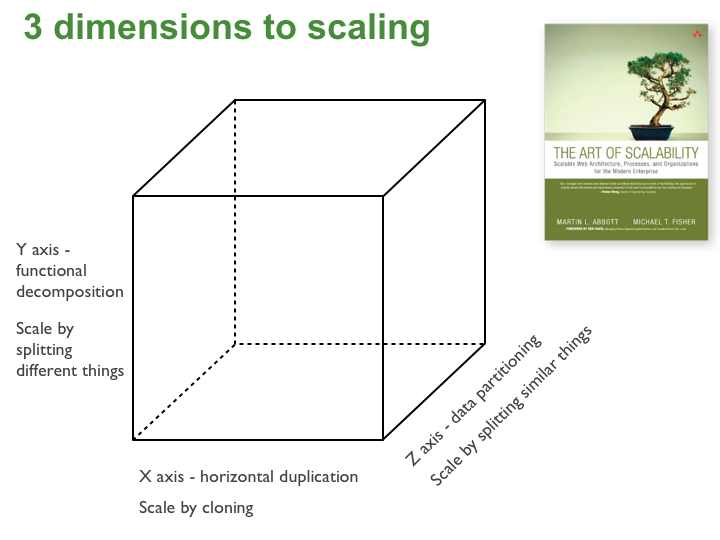
\includegraphics{img/ScaleCude.jpg}
\caption{Scaling Cube}
\end{figure}

Ahogy a képen is látható a meghatározó felbontási fogalmak, az adat
menti felbontás, a tetszőleges fogalom menti felbontás, illetve a
klónozás.

\subsection{Adat menti felbontás}\label{adat-menti-felbontuxe1s}

Az adat menti felbontás annyit tesz, hogy a szolgáltatásokat annak
megfelelően bontjuk fel, hogy milyen erőforrással dolgoznak, vagy
konkrétan egy adattal kapcsolatos összes funkciót egy helyen készítünk
el.

Példa: Erőforrás szerinti felbontás ha külön található szolgáltatás,
amivel az adatbázis műveleteket hajtjuk égre, és külön van olyan is, ami
csak a HTTP kéréseket szolgálja ki. Az egy adatra épülő módszernél pedig
alapul vehetünk egy olyan példát, ahol mondjuk egy szolgáltatás az
összes adminisztrátori funkciót látja el, míg más szolgáltatások a
más-más kategóriába eső felhasználók műveleteit hajtják végre.

Mivel a mikro szolgáltatások elve a hardvert is megosztja nem csak a
szoftvert, ezért az erőforrás szerinti szétválasztás kissé
értelmetlennek tűnhet, azonban a különböző platformok különbüző
erőforrásait megéri külön szolgáltatásként kezelni.

\subsection{Fogalmi felbontás}\label{fogalmi-felbontuxe1s}

A tetszőleges fogalom menti felbontás annyit tesz hogy elosztott
rendszert hozunk létre tetszőleges funkcionalitás szerint. Erre épít a
mikro szolgáltatás architektúra is, mivel a lényege pont az egyes
funkciók atomi felbontása.

Példa: Adott egy könyvtár nyilvántartó rendszere, és ezt akarjuk
fogalmanként szétvágni. Külön-külön lehet szolgáltatást csinálni a
keresésnek, indexelésnek, foglalásnak, kivett könyvek nyilvántartásának,
böngészésre, könyvek adatainak tárolására, és kiolvasására, és ehhez
hasonló funkciókra. Ezekkel a szétválasztásokkal a könyvtár működését
kis részekre bontottuk, és ezek egy-egy kis szolgáltatásként könnyen
elérhetők.

\subsection{Klónozás}\label{kluxf3nozuxe1s}

A harmadik módszer arra tér ki, hogy hogyan lehet egy architektúrát
felosztani, hogy skálázható legyen. Itt a klónozhatóság, avagy az egymás
melleti kiszolgálás motivál. Ez a mikro szolgáltatásoknál kell, hogy
teljesüljön, mivel adott esetben egy terhelés elosztó alatt tudnunk kell
definiálni több példányt is egy szolgáltatásból. Azért szükséges a
skálázhatóság a mikro szolgáltatások esetén, mivel kevés hardver mellett
is hatékonyan kialakítható az architektúra, de könnyen lehet szűk
keresztmetszetet létrehozni, amit skálázással könnyen megkerülhetünk.

\section{Architektúrális mintákhoz való
viszonya}\label{architektuxfaruxe1lis-mintuxe1khoz-valuxf3-viszonya}

Mint korábban láthattuk vannak bizonyos telepítési módszerek, amik
mentén szokás a mikro szolgáltatásokat felépíteni. Van aki az
architektúrális tervezési minták közé sorolja a mikro szolgáltatás
architektúrát, de nem könnyű meghatározni, hogy hogyan is alkot önnáló
mintát. Nagyon sok lehetőség van a mikro szolgáltatásokban, és leginkább
más architektúrákkal együtt használva lehet hatékonyan és jól használni.

Nézzünk meg két felhasználható architektúrális mintát:

\subsection{Pipes and Filters}\label{pipes-and-filters}

A Pipes and fileter architektúrális minta\citep{pipes-pattern} lényege,
hogy a funkciókra bontott architektúrát az elérni kívánt végeredmény
érdekében különböző módokon összekötjük. Ebben a módszerben az adat
folyamatosan áramlik az egyes alkotó elemek között, és lépésről lépésre
alakul ki a végeredmény. Elég olcsón kivitelezhető architektúrális
minta, mivel csupán sorba kell kötni hozzá az egyes szolgáltatásokat,
azonban nehezen lehet optimalizálni, és könnyen lehet, hogy olyan részek
lesznek a feldolgozás közben, amik hátráltatják a teljes folyamatot.

\subsection{Publish/Subscribe}\label{publishsubscribe}

Egy másik elosztott rendszerekhez kitallált minta a
subscriber/publisher\citep{pub-subscribed}, amely arra alapszik, hogy
egy szolgáltatásnak szüksége van valamilyan adatra vagy funkcióra, és
ezért feliratkozik egy másik szolgáltatásra. Ennek az lesz az eredménye,
hogy bizonyos szolgáltatások bizonyos más szolgáltatásokhoz fognak
kötődni, és annak megfelelően fognak egymással kommunikálni, hogy milyen
feladatot kell végrehajtaniuk.

\subsection{Esemény alapú
architektúra}\label{esemuxe9ny-alapuxfa-architektuxfara}

Az esemény alapú architektúrákat\citep{event-driven-pattern} könnyen
kalakíthatjuk, ha egy mikro szolgáltatásokból álló rendszerben olyan
alkalmazásokat és kompoenenseket fejlesztünk ahol eseményeken keresztül
kommunikálnak az egyes elemek. Ezzel a nézettel olyan mikro
szolgáltatásokból kialakuló struktúrát lehet összeépíteni, ahol a kis
egységek szükség szerint kommunikálnak, és a kommunikáció egy jól
definiált interfészen kerseztül történik.

\section{Eltérések a szolgáltatás orientált
architektúrától}\label{eltuxe9ruxe9sek-a-szolguxe1ltatuxe1s-orientuxe1lt-architektuxfaruxe1tuxf3l}

A szolgáltatás orientált architektúra nagyon hasonló a mikro
szolgáltatásokhoz, azonban utóbbi esetén a lényeg az, hogy minnél kisebb
alkotó elemekre bontsuk szét a rendszert és akár alkalmazásokat is, míg
előbbi több alkalmazát köt össze hálózati kapcsolaton keresztül, és
ezeket szolgáltatja ki. Bizonyos értelemben a mikro szolgáltatás
architektúra a szolgáltatás orientált architektúra finomítása.

\section{Példák mikro szolgáltatásokat használó
alkalmazásokra}\label{puxe9lduxe1k-mikro-szolguxe1ltatuxe1sokat-hasznuxe1luxf3-alkalmazuxe1sokra}

Amazon - minden Amazon-nal kommunikáló eszköz illetve az egyes funkciók
implementációja is szolgáltatásokra van szedve, és ezeket hívják az
egyes funkciók (vm indítás, törlés, mozgatás, stb.)

eBay - Különböző műveletek szerint van felbonva a a funkcionalitás, és
ennek megfelelően külön szolgáltatásként érhető el a fizetés,
megrendelés, szállítási információk, stb.

NetFlix - A nagy terhelést elkerülendő bizonyos streaming
szolgáltatásokat átlalakítottak, hogy a mikro szolgáltatás architektúra
szerint működjön.

Archivematica\citep{archivematica} - Egy Fájlkezelő rendszer, amiben
mikro szolgáltatásoknak megfelelően alakították ki a plugin-ként
használható funkciókat.

\chapter{Mikro szolgáltatások előnyei és
hátrányai}\label{mikro-szolguxe1ltatuxe1sok-elux151nyei-uxe9s-huxe1truxe1nyai}

Ahogy minden architektúrális mintának, a mikro szolgáltatásoknak is
vannak előnyei, amik indokoltá teszik a minta használatát, és vannak
hátrányai, amiket mérlegelnünk kell a tervezés folyamán.

\section{\texorpdfstring{Előnyök
\citep{microservices}}{Előnyök {[}@microservices{]}}}\label{elux151nyuxf6k-microservices}

\subsection{Könnyű fejleszteni}\label{kuxf6nnyux171-fejleszteni}

Mivel kis részekre van szedve az alkalmazásunk, a fejlesztést akát több
csapatnak is ki lehet osztani, hogy az alkalmazás részeit alkossák meg,
hiszen önállóan is életképesek a szolgáltatások. Az egyes szolgáltatások
nem rendelkeznek túl sok logikával, így ez kis feladatokat csinál, és
könnyebben kezelhető.

\subsection{Egyszerűen
megérthető}\label{egyszerux171en-meguxe9rthetux151}

Egy szolgáltatás nagyon kis egysége a teljes alkalmazásnak, így könnyen
megérthető. Kevés technológia, és kevés kód áll rendelkezésre egy
szolgáltatásnál, így gyorsan beletanulhat egy új fejlesztő a munkába.

\subsection{Könnyen kicserélhető, módosítható,
telepíthető}\label{kuxf6nnyen-kicseruxe9lhetux151-muxf3dosuxedthatuxf3-telepuxedthetux151}

A szolgáltatások önnálóak, így az azonos interfésszel rendelkező
szolgáltatásra bármikor kicserélhető, illetve módosítható ha megmaradnak
a korábbi funkciók. A mikor szolgáltatás telepítése is egyszerű, mivel
csak kevés környezeti feltétele van, hogy egy ilyen kis máretű progam
működni tudjon.

\subsection{Jól skálázható}\label{juxf3l-skuxe1luxe1zhatuxf3}

Mivel sok kis részletből áll az alkalmazásunk, nem szükséges minden
funkciónkhoz növelni az erőforrások allokációját, hanem kis
komponensekhez is lehet rendelni több erőforrást.

\subsection{Támogatja a kevert
technológiákat}\label{tuxe1mogatja-a-kevert-technoluxf3giuxe1kat}

Az egyik legnagyobb ereje ennek az architektúrának, hogy képes egy
alkalmazáson belül kevert technológiákat is használni. Mivel egy jól
definiált interfészen keresztül kommunikálnak a szolgáltatások, ezért
mindegy milyen technológia van mögötte, amíg ki tudja szolgálni a
feladatát. Ennek megfelelően El tudunk helyezni egy Linux-os
környezetben használt LDAP-ot, és egy Windows-os környezetben használt
Active Directory-t, és minden gond nélkül használni is tudjuk az
interfész segítségével.

\section{\texorpdfstring{Hátrányok
\citep{micro-disadv}}{Hátrányok {[}@micro-disadv{]}}}\label{huxe1truxe1nyok-micro-disadv}

\subsection{Komplex rendszer alakul
ki}\label{komplex-rendszer-alakul-ki}

Mivel minden funkcióra saját szolgáltatást csinálunk, nagyon sok lesz az
elkülönülő elem, és a teljes rendszer egyben tartása nagyon nehéz
feladattá válik. Mivel fontos a szolgáltatások együttműködése, a sok
interfésznek ismernie kell egymást, és fenn kell tartani a
konzisztenciát minden szolgáltatásnak.

\subsection{Nehezen kezelhető az elosztott
rendszer}\label{nehezen-kezelhetux151-az-elosztott-rendszer}

A mikro szolgáltatások architektúra egy elosztott rendszert ír le, és
mint minden elosztott rendszer ez is bonyolultabb lesz tőle. Elosztott
rendszereknél figyelni kell az adatok konzisztenciáját, a kommunikáció
plusz feladatot ad minden szolgáltatás fejlesztőjének, és folyamatosan
együtt kell működni a többi szolgáltatás fejlesztőjével.

\subsection{Plusz munkát jelént az aszinkron üzenet
fogadás}\label{plusz-munkuxe1t-jeluxe9nt-az-aszinkron-uxfczenet-fogaduxe1s}

Mivel egy szolgáltatás egyszerre több kérést is ki kell hogy szolgáljon
egyszerűbb ha aszinkron módon működik. Ezt azonban mindig le kell
implementálni, és az aszinkron üzenetek bonyolítják az adatok kezelését.

\subsection{Kód duplikátumok
kialakulása}\label{kuxf3d-duplikuxe1tumok-kialakuluxe1sa}

Amikor nagyon hasonló (kis részletben eltérő) szolgáltatásokat
csinálunk, megesik, hogy ugyan azt a kódot többször fel kell
használnunk, és ezzel kód, és adat duplikátumok keletkeznek, amiket le
kell kezelnünk.

\subsection{Interfészek
fixálódnak}\label{interfuxe9szek-fixuxe1luxf3dnak}

A fejlesztés folyamán a szolgáltatásokhoz rendelt interfészek
fixálódnak, és ha módosítani akarunk rajta, akkor több szolgáltatásban
is meg kell változtatni az interfészt.

\subsection{Nehezen tesztelhető
egészben}\label{nehezen-tesztelhetux151-eguxe9szben}

Mivel sok kis részletből rakódik össze a nagy egész alkalmazás, a
tesztelési fázisban kell olyan teszteket is végezni, ami a rendszer
egészét, és a kész alkalmazást teszteli. Egy ilyen teszt elksézítése
bonyolult lehet, és plusz feladatot ad a sok szolgáltatás külön-külön
fordítása, és telepítése is.

\section{Összehasonlítva a monolitikus
architektúrával}\label{uxf6sszehasonluxedtva-a-monolitikus-architektuxfaruxe1val}

A mirco-service architektúrák a monolitikus architektúra ellentetjei,
melyben az erőforrások központilag vannak kezelve, és minden funkció egy
nagy interfészen keresztül érhető el. A monolitikus architektúra
egyszerűen kiépíthető, könnyű tervezni és fejleszteni, azonban nehezen
lehet kicserélni, nem elég robosztus, és nehezen skálázható, mivel az
erőforrásokat közösen kezelik a funkciók.

Ezzel ellenzétben a mikro szolgáltatás architektúrát ugyan nehezen lehet
megtervezni, hiszen egy elosztott rendszert kell megtervezni, ahol az
adatátviteltől kezdve az erőforrás megosztáson keresztül semmi sem
egyértelmű, viszont a későbbi tovább fejlesztés sokkal egyszerűbb, mivel
külön csapatokat lehet rendelni az egyes szolgáltatásokhoz, és könnyen
integrálhatók kicserélhetők az alkotó elemek. Mivel sok kis egységből
áll, könnyebben lehet úgy skálázni a rendszert, hogy ne pazaroljuk el az
erőforrásainkat, és ugyanakkor a kis szolgáltatások erőforrásokban is el
vannak különítve, így nem okoz gondot, hogy fel vagy le skálázzunk egy
szolgáltatást. Ennek az a hátránya, hogy le kell kezelni a skálázáskor a
közös erőforrásokat.(Például ha veszünk egy autentikációs szolgáltatást,
akkor ha azt fel skálázzuk, meg kell tartanunk a felhasználók listáját,
így duplikálni kell az adatbázist, és fenntartani a konzisztenciát)
Ugyan csak előnye a mirco-service architektúrának, hogy különböző
technológiákat lehet keverni vele, mivel az egyes szolgáltatások
különböző technológiákkal különböző platformon is futhatnak.

\chapter{Technológiai
áttekintés}\label{technoluxf3giai-uxe1ttekintuxe9s}

Az integrációhoz olyan technológiákat lehet használni, melyek lehetővé
teszik az egyes szolgáltatások elkülönült működését. Ahhoz, hogy jó
technológiákat válasszunk, mindeképpen ismernünk kell az igényeket,
mivel a technológiák széles köre áll rendelkezésünkre. Fontos szem előtt
tartani pár általános érvényű szabályt is\citep{micro-golden}, ami a
mikroszolgáltatások helyes működéséhez kell. Ezek pedig a következők:

\begin{itemize}
\tightlist
\item
  Modulárisan szétválasztani a szolgáltatásokat
\item
  Legyenek egymástól teljesen elkülönítve
\item
  Legyen jól definiált a szolgáltatások kapcsolata
\end{itemize}

A következő feladatokra kellenek technológiák: * Hogyan lehet
feltelepíteni egy önálló szolgáltatást? (telepítés) * Hogyan lehet
összekötni ezeket a szolgáltatásokat? (automatikus környezet felderítés)
* Hogyan lehet fenntartani, változtatni a szolgáltatások környezetét?
(integrációs keretrendszer) * Hogyan lehet skálázni a szolgáltatást?
(skálázás) * Hogyan lehet egységesen használni a skálázott
szolgáltatásokat? (load balance, konzisztencia fenntartás) * Hogyan
lehet virtualizáltan ezt kivitelezni? (virtualizálás) * A meglévő
szolgáltatásokat hogyan tartsuk nyilván? (service registy) * Hogyan
figyeljük meg az alkalmazást működés közben (monitorozás, loggolás)

\section{Telepítési
technológiák}\label{telepuxedtuxe9si-technoluxf3giuxe1k}

A microservice-eket valamilyen módon létre kell hozni, egy hosthoz kell
rendelni, és az egyes elemeket össze kell kötni. A szolgáltatások
telepítéséhez olyan technológiára van szükség amivel könnyen elérhetünk
egy távoli gépet, és könnyen kezelhetsük az ottani erőforrásokat. Ehhez
a legkézenfekvőbb megoldás a Linux rendszerek esetén az SSH kapcsolaton
keresztül végrehajtott Bash parancs, de vannak eszközök, amikkel ezt
egyszerűbben és elosztottabban is megtehetjük.

\begin{itemize}
\item
  \textbf{Jenkins}\citep{jenkins}: A Jenkins egy olyan folytonos
  integráláshoz kifejlesztett eszköz, mellyel képesek vagyunk különböző
  funkciókat automatizálni, vagy időzítetten futtani. A Jenkins egy Java
  alapú webes felülettel rendelkező alkalmazás, amely képes bash
  parancsokat futtatni, Docker konténereket kezelni, build-eket
  futtatni, illetve a hozzá fejlesztett plugin-eken keresztül, szinte
  bármire képes. Támogatja a fürtözést is, így képesek vagyunk Jenkins
  slave-eket létrehozni, amik a mester szerverrel kommunikálva végzik el
  a dolgukat. A microservice architektúrák esetén alkalmas a
  szolgáltatások telepítésére, és tesztelésére.
\item
  \textbf{ElasticBox}\citep{elasticbox}: Egy olyan alkalmazás, melyben
  nyilvántarthatjuk az alkalmazásainkat, és könnyen egyszerűen
  telepíthetjük őket. Támogatja a konfigurációk változását, illetve
  számos technológiát, amivel karban tarthatjuk a környezetünket.
  (Docker, Puppet, Ansible, Chef, stb) Együtt működik különböző cloud
  megoldásokkal, mint az AWS, vSphere, Azure, és más környezetek.
  Hasonlít a Jenkins-re, csupán ki van élezve a microservice
  architektúrák vezérlésére. (Illetve fizetős a Jenkins-el ellentétben)
  Mindent végre tud hajtani ami egy microservice alkalmazáshoz
  szükséges, teljes körű felügyeletet biztosít.
  \citep{jenkins-elasticbox}
\item
  \textbf{Kubernetes}\citep{kubernetes}: A Kubernetes az ElasticBox egy
  opensource változata, ami lényegesen kevesebbet tud, azonban
  ingyenesen elérhető. Ez a projekt még nagyon gyerekcipőben jár, így
  nem tudom felhasználni a félév során.
\end{itemize}

Egyéb lehetőség, hogy a fejlesztő készít magának egy olyan szkriptet,
ami elkészíti számára a micro-service architektúrát, és lehetővé teszi
az elemek dinamikus kicserélését. (ad-hoc megoldás)

\section{Környezet felderítési
technológiák}\label{kuxf6rnyezet-felderuxedtuxe9si-technoluxf3giuxe1k}

Az egyes szolgáltatásoknak meg kell találniuk egymást, hogy megfelelően
működhessen a rendszer, azonban ez nem mindig triviális, így szükség van
egy olyan alkalmazásra, amivel felderíthetjük az aktív szolgáltatásokat.

\begin{itemize}
\tightlist
\item
  \textbf{Consul}\citep{consul}: A Hashicorp szolgáltatás felderítő
  alkalmazása, amely egy kliens-szerver architektúrának megfelelően
  megtalálja a környezetében lévő szolgáltatásokat, és figyeli az
  állapotukat (ha inaktívvá válik egy szolgáltatás a Consul észre
  veszi). Ez az alkalmazás egy folyamatosan választott mester node-ból
  és a többi slave node-ból áll. A mester figyeli az alárendelteket, és
  kezeli a kommunikációt. Egy új slave-et úgy tudunk felvenni, hogy a
  consul klienssel kapcsolódunk a mesterre. Ha automatizáltan tudjuk
  vezényelni a feliratkozást, egy nagyon erős eszköz kerül a kezünkbe,
  mivel eseményeket küldhetünk a szervereknek, és ezekre különböző
  feladatokat hajthatunk végre.
\end{itemize}

\section{Integrációs
keretrendszerek}\label{integruxe1ciuxf3s-keretrendszerek}

A telepítéshez és a rendszer állapotának a fenntartásához egy olyan
eszköz kell, amivel gyorsan egyszerűen végrehajthatjuk a
változtatásainkat, és ha valamit változtatunk egy szolgáltatásban, akkor
az összes hozzá hasonló szolgáltatás értesüljön a változtatáról, vagy
hajtson végre ő maga is változtatást.

\begin{itemize}
\item
  \textbf{Puppet}\citep{puppet}: Olyan nyilt forrású megoldás, amellyel
  leírhatjuk objektum orientáltan, hogy milyen változtatásokat akarunk
  elérni, és a Puppet elvégzi a változtatásokat. Automatizálja a
  szolgáltatás változtatásának minden lépését, és egyszerű gyors
  megoldást szolgáltatat a komplex rendszerbe integráláshoz.
\item
  \textbf{Chef}\citep{chef}: A Chef egy olyan konfiguráció menedzsment
  eszköz ami nagy mennyiségű szerver számítógépet képes kezelni,
  fürtözhető, és megfigyeli az alá szervezett szerverek állapotát.
  Tartja a kapcsolatot a gépekkel, és ha valamelyik konfiguráció nem
  felel meg a definiált repectkönynek (amiben definiálhatjuk az elvárt
  környezeti paramétereket) akkor változtatásokat indít be, és eléri,
  hogy a szerver a megfelelő konfigurációval rendelkezzen. Népszerű
  konfiguráció menedzsment eszköz, amiz könnyedén használhatunk
  integrációhoz, illetve a szolgáltatások cseréjéhez, és
  karbantartásához.
\item
  \textbf{Ansible}\citep{ansible}: A Chef-hez hasonlóan képes
  változtatásokat eszközölni a szerver gépeken egy SSH kapcsolaton
  keresztül, viszont a Chef-el ellentétben nem tartja a folyamatos
  kapcsolatot. Az Ansible egy tipikusan integrációs célokra
  kifejlesztett eszköz, amelyhez felvehetjük a gépeket, amiken
  valamilyen konfigurációs változtatást akarunk végezni, és egy
  ``playbook'' segítségével leírhatjuk milyen változásokat kell
  végrehajtani melyik szerverre. Könnyen irányíthatjuk vele a
  szolgáltatásokat, és definiálhatunk szolgáltatásonként egy playbook-ot
  ami mondjuk egy fürtnyi szolgáltatást vezérel. Ez az eszköz hasznos
  lehet, ha egy szolgáltatásnak elő akarjuk készíteni a környezetet.
\item
  \textbf{SaltStack}\citep{saltstack}: A SaltStack nagyon hasonlít a
  Chef-re, mivel ez a termék is széleskörű felügyeletet, és konfiguráció
  menedzsment-et kínál számunkra, amit folyamatos kapcsolat
  fenntartással, és gyors kommunikációval ér el. Az Ansible-höz nagyon
  hasonlóan konfigurálható (nem lennék meglepve ha azt használná a
  háttérben), szintén ágens nélküli kapcsolatot tud létesíteni, és a
  Chef-hez hasonlóan több 10 ezer gépet tud egyszerre karbantartani.
\end{itemize}

\section{Skálázási
technológiák}\label{skuxe1luxe1zuxe1si-technoluxf3giuxe1k}

A microservice architektúrák egyik nagy előnye, hogy az egyes funkciókra
épülő szolgáltatásokat könnyedén lehet skálázni, mivel egy load
balancert használva csupán egy újabb gépet kell beszervezni, és máris
nagyobb terhelést is elbír a rendszer. Ahhoz hogy ezt kivitelezni
tudjuk, szükségünk van egy terhelés elosztóra, és egy olyan logikára,
ami képes megsokszorozni az erőforrásainkat. Cloud-os környezetben ez
könnyen kivitelezhető, egyébként hideg tartalékban tartott gépek
behozatalával elérhető. Sajnálatos módon általános célú skálázó eszköz
nincsen a piacon, viszont gyakran készítenek maguknak saját logikát a
nagyobb gyártók.

\begin{itemize}
\tightlist
\item
  \textbf{Elastic Load Balancer}\citep{elastic-load-balance}: Az Amazon
  AWS-ben az ELB avagy rugalmas terhelés elosztó az, ami ezt a célt
  szolgálja. Ennek a szolgáltatásnak az lenne a lényege, hogy segítse az
  Amazon Cloud-ban futó virtuális gépek hibatűrését, illtve egységbe
  szervezi a különböző elérhetőségi zónákban lévő gépeket, amivel
  gyorsabb elérést tudunk elérni. Mivel ez a szolgáltatás csupán az
  Amazon AWS-t felhasználva tud működni, nem megfelelő általános célra,
  azonban ha az Amazon Cloud-ban építjük fel a microservice
  architektúránkat, akkor erős eszköz lehet számunkra.
\end{itemize}

\section{Terhelés elosztás}\label{terheluxe9s-elosztuxe1s}

A microservice architektúrának egyik fontos eleme a terhelés elosztó,
vagy valamilyen fürtözést lehetővé tevő eszköz. Ez azért fontos, mert
egy egységes interfészt tudunk kialakítani a szolgáltatásaink elérésére,
és könnyíti a skálázódást a szolgáltatások mentén.

\begin{itemize}
\item
  \textbf{HAProxy}\citep{haproxy} \citep{LB-haproxy}: Egy magas
  rendelkezésre állást biztosító, és megbízhatóságot növelő terhelés
  elosztó eszköz. Konfigurációs fájlokon keresztül megszervezhetjük,
  hogy mely gépet hogyan érjünk el, milyen IP címek mely
  szolgáltatásokhoz tartoznak, illetve round robin módon osztja szét a
  kéréseket az egyes szerverek között. Ez az eszköz csak és kizárólak a
  HTTP TCP kéréseket tudja elosztani, de egyszerű könnyen telepíthető,
  és könnyen kezelhető (ha nem dinamikusan változnak a fürtben lévő
  gépek, mert ha igen akkor szükséges egy mellékes frissítő logika is)
\item
  \textbf{ngnix}\citep{nginx}: Az Nginx egy nyilt forráskódú web
  kiszolgáló és reverse proxy szerver, amivel nagy méretű rendszereket
  kezelhetünk, és segít az alkalmazás biztonságának megörzésében. A
  kiterjesztett változatával (Nginx Plus) képesek lehetünk a terhelés
  elosztásra, és alkalmazás telepítésre. Nem teljesen a proxy szerver
  szerepét váltja ki, de képes elvégezni azt.
\end{itemize}

\section{Virtualizációs
technológiál}\label{virtualizuxe1ciuxf3s-technoluxf3giuxe1l}

A microservice architektúrák kialakításánál nagy előnyt jelenthet, ha
valamilyen virtualizációt használunk fel a környezet kialakításához.
Virtualizált környezetben könnyebb a telepítés, skálázás, és a
monitorozás is egyszerűbb lehet.

\begin{itemize}
\item
  \textbf{Docker}\citep{docker}: Egy konténer virtualizációs eszköz,
  amelynek segítségével egy adott kernel alatt több különböző
  környezettel rendelkező alkalmazásokat futtató környezetet hozhatunk
  létre. A Docker egy szeparált fájlrendszert hoz létre a host gépen, és
  abban hajt végre műveleteket. Készíthetünk vele előre elkészített
  alkalmazás környezeteket, és szolgáltatásokat, ami ideálissá teszi
  microservice architektúrák létrehozásánál. A Docker konténerek
  segítségével egyszerűen telepíthetjük, skálázhatjuk, és fejleszthetjük
  a rendszert.
\item
  \textbf{libvirt}\citep{libvirt}: Többféle virtualizációs
  technológiával egyűtt működő eszköz, amivel könnyedén irányíthatjuk a
  virtuális gépeket, és a virtualizálás komolyabb részét el
  absztrahálja. Támogat KVM-em, XEN-t, VirtualBox-ot LXC, és sok más
  virtualizáló eszköt. Ezzel az eszközzel a környezet kialakítását
  szabhatjuk meg, tehát a hardware-eserőforrások megosztásában nyújt
  nagy segítséget.
\item
  \textbf{kvm}\citep{kvm}: A KVM egy kernel szintű virtualizációs
  eszköz, amivel virtuális gépeket tudunk készíteni. Processzor szintjén
  képes szétválasztani az erőforrásokat, és ezzel szeparált
  környezeteket létrehozni. Virtualizál a processzoron kívül hálózati
  kártyát, háttértárat, grafikus meghajtót, és sok mást. A KVM egy nyilt
  forrűskódú projekt és létrehozhatunk vele Linux és Windows gépeket is
  egyaránt.
\item
  \textbf{Akármilyen cloud}: Ha virtualizációról beszélünk, akkor adja
  magát hogy a CLoud-os környezeteket is ide értsük. Egy microservice
  architektúrájú programot a legcélszerűbb valamilyen Cloud-os
  környezetben létrehozni, mivel egy ilyen környezetnek definiciója
  szerint tartalmaznia kell egy virtualizációs szintet, megosztott
  erőforrásokat, monitorozást, és egyfajta leltárat a futó példányokról.
  Ennek megfelelően a microservice architektúra minden környezeti
  feltételét lefedi, csupán a szolgáltatásokat, business logikát, és az
  interfészeket kell elkészítenünk. Jellemzően a Cloud-os környezetek
  tartalmaznak terhelés elosztást, és skálázási megoldást is, amivel
  szintén erősítik a szolgáltatás alapú architektúrákat. Ilyen környezet
  lehet az Amazon, Microsoft Azure, Google App Engine, OpenStack, és
  sokan mások.
\end{itemize}

\section{\texorpdfstring{Service registy-k
\citep{service-registry-pattern}}{Service registy-k {[}@service-registry-pattern{]}}}\label{service-registy-k-service-registry-pattern}

Számon kell tartani, hogy milyen szolgáltatások elérhetők, milyen címen
és hány példányban az architektúránkban, és ehhez valamilyen
szolgáltatás nyilvántartási eszközt kell használnunk.

\begin{itemize}
\item
  \textbf{Eureka}\citep{eureka-glance}: Az Eureka a Netflix fejlesztése,
  egy AWS környezetben működő terhelés elosztó alkalmazás, ami figyeli a
  felvett szolgáltatásokat, és így mint nyilvántartás is megfelelő. A
  kommunikációt és a kapcsolatot egy Java nyelven írt szerver és kliens
  biztosítja, ami a teljes logikát megvalósítja. EGyütt működik a
  Netflix álltal fejlesztett Asgard nevezetű alkalmazással ami az AWS
  szolgáltatásokhoz való hozzáférést segíti. Ugyan ez az eszköz erősen
  optimalizált az Amazon Cloud szolgáltatásaihoz, de a leírás alapján
  megállja a helyét önállóan is. Mivel nyilt forráskódú, mintát
  szolgáltat egyéb alkalmazásoknak is.
\item
  \textbf{Consul}: Korábban már említettem ezt az eszközt, mivel abban
  segít, hogy felismerjék egymást a szolgáltatások. A kapcsolatot
  vizsgáló és felderítő logikán kívül tartalmaz egy nyilvántartást is a
  beregisztrált szolgáltatásokról, amiknek az állapotát is
  vizsgálhatjuk.
\item
  \textbf{Apache Zookeeper}\citep{zookeeper}: A Zookeeper egy
  központosított szolgáltatás konfigurációs adatok és hálózati adatok
  karbantartására, ami támogatja az elosztott működést, és a szerverek
  csoportosítását. Az alkalmazást elosztott alkalmazás fejlesztésre, és
  komplex rendszer felügyeletére és telepítés segítésére tervezték. A
  conzulhoz hasonlóan működik, és a feladata is ugyan az.
\end{itemize}

\section{\texorpdfstring{Monitorozás, loggolás
\citep{micro-service-monitoring}
\citep{microservice-monitoring}}{Monitorozás, loggolás {[}@micro-service-monitoring{]} {[}@microservice-monitoring{]}}}\label{monitorozuxe1s-loggoluxe1s-micro-service-monitoring-microservice-monitoring}

Ha már megépítettük a microservice architektúrát, akkor meg kell
bizonyosodnunk róla, hogy minden megfelelően működik, és minden rendben
zajlik a szolgáltatásokkal. Ehhez többféle módon és többféle eszközzel
is hozzáférhetünk, mivel az alkalmazás hibákat egy log szerver, a
környezeti problémákat egy monitorozó szerver tudja megfelelően
megmutatni számunkra.

\begin{itemize}
\item
  \textbf{Zabbix}\citep{zabbix}: A Zabbix egy sok területen felhasznált,
  több 10 ezer szervert párhuzamosan megfigyelni képes, akármilyen
  adatot tárolni képes monitorozó alkalmazás, ami képes elosztott
  működésre, és virtuális környezetekben jól használható. Ágens nélküli
  és ágenses adatgyűjtésre is képes, és az adatokat különböző módokon
  képes megjeleníteni (földrajzi elhelyezkedés, gráfos megjelenítés,
  stb.). Nem egészen a microservice architektúrákhoz lett kialakítva, de
  egy elég általános eszköz, hogy felhasználható legyen ilyen célra is.
\item
  \textbf{Kibana\citep{kibana} + LogStash}\citep{logstash}: A Kibana egy
  ingyenes adatmegjelenítő és adatfeldolgozó eszköz, amit az
  elasticsearch fejlesztett ki, és a logstash pedig egy log server,
  amivel tárolhatjuk a loggolási adatainkat, és egyszerűen kereshetünk
  benne. Kifejezetten adatfeldolgozásra szolgál mind a két eszköz, és
  közvetlenül együttműködnek az elasticsearch alkalmazással.
\item
  \textbf{Sensu}\citep{sensu}: A Sensu egy egyszerű monitorozó eszköz,
  amivel megfigyelhetjük a szervereinket. Támogatja Ansible Chef, Puppet
  használatát, és támogatja a Plugin szerű bővíthetőséget. A felülete
  letisztult és elég jó áttekintést ad a szerverek állapotáról. Figyel a
  dinamikus változásokra, és gyorsan lekezeli a változásokkal járó
  riasztásokat. Ezek a tulajdonságai teszik a Cloud-okban könnyen és
  hatékonyan felhasználhatóvá.
\item
  \textbf{Cronitor}\citep{cronitor} \citep{cron-monitoring}: Ez a
  monitorozó eszköz mikró-szolgáltatások és cron job-ok megfigyelésére
  lett kifejlesztve, HTTP-n keresztül kommunikál, és a szologáltatások
  állapotát figyeli. Nem túl széleskörű eszköz, azonban ha csak a
  szolgáltatások állapota érdekel hasznos lehet, és segíthet a Service
  Registry képzésében is.
\item
  \textbf{Ruxit}\citep{ruxit} \citep{ruxit-monitoring}: Egy
  Cloud-osított monitorozó eszköz, amivel teljesítmény monitorozást,
  elérhetőség monitorozást, és figyelmeztetés küldést végezhetünk. Az
  benne a különleges, hogy mesterséges intelligencia figyeli a
  szervereket, és kianalizálja a szerver állapotát, és a
  figyelmeztetéseket is követi. Könnyen skálázható, és használat alapú
  bérezése van. Ez a választás akkor jön jól, ha olyan feladatot szánunk
  az alkalmazásunknak, ami esetleg időben nagyon változó terhelést
  mutat, és az itt kapot riasztások szerint akarunk skálázni.
\end{itemize}

\chapter{Kommunikációs
módszerek}\label{kommunikuxe1ciuxf3s-muxf3dszerek}

A szolgáltatások közötti kommunikáció nincs lekötve de jellemző a
REST-es API, vagy a webservice-re jellemző XML alapú
kommunikáció\citep{rest-soap}.

\section{Technológiák}\label{technoluxf3giuxe1k}

A kommunikáció megtervezéséhez egy jó leírást olvashatunk az Nginx egyik
cikkében\citep{micro-communication}. Ez a cikk leírja, fontos előre
eltervezni, hogy a szolgáltatások egyszerre több másik szolgáltatással
is kommuniikálnak vagy nem, illetve szinkron vagy aszinkron módon
akarunk-e kommunikálni. A cikk kifejti, hogy az egyes technológiák
hogyan használhatók jól, és hogyan lehet várakoztatási sorral javítani a
kiszolgáláson.

\subsection{\texorpdfstring{REST
(HTTP/JSON)\citep{microservices-light}:}{REST (HTTP/JSON){[}@microservices-light{]}:}}\label{rest-httpjsonmicroservices-light}

A RESTful kommunikáció egy HTTP feletti kommunikációs fajta, aminek az
alapja az erőforrások megjelölése egyedi azonosítókkal, és hálózaton
keresztül műveletek végzése a HTTP funkciókat felhasználva. Ez a módszer
napjainkban nagyon népszerű, mivel egyszerű kivitelezni, gyakorlatilag
minden programozási nyelv támogatja, és nagyon egyszerűen építhetünk
vele interfészeket. Az üzenetek törzsét a JSON tartalom adja, ami egy
kulcs érték párokból álló adatstruktúra, és sok nyelv témogatj az
objektumokkal való kommunikációt JSON adatokon keresztül. Mikro
szolgáltatások esetén az aszinkron változat használata az
előnyösebb\citep{rest-async}, mivel ekkor több kérést is ki tudunk
szolgálni egyszerre, és a szolgáltatásoknak nem kell várniuk a szinkron
üzenetek kiszolgálására.

\subsection{\texorpdfstring{SOAP
(HTTP/XML)\citep{soap}:}{SOAP (HTTP/XML){[}@soap{]}:}}\label{soap-httpxmlsoap}

A szolgáltatás alapú architektúrákban nagyon népszerű, mivel tetszőleges
interfészt definiálhatunk, és le lehet vele képezni objektumokat is.
Kötött üzenetei vannak, amiket egy XML formátumu üzenet ír le. Ebben az
esetben nem erőforrásokat jelölnek az URL-ek, hanem végpontokat, amik
mögött implementálva van a funkcionalitás. Ennek a kommunikációs
módszernek az az előnye, hogy jól bejáratot, széleskörben használt
technológiáról van szó, amit jól lehet használni objektum orientált
nyelvek közötti adatátvitelre. Hátránya, hogy nagyobb a sávszélesség
igénye, és lassabb a REST-es megoldásnál. Létezik szinkron és aszinkron
megvalósítása is és mivel ez a kommunikációs fajta is HTTP felett
történik, a REST-hez hasonló okokból az aszinkron változat a célszerűbb.

\subsection{\texorpdfstring{Socket
(TCP)\citep{socket}:}{Socket (TCP){[}@socket{]}:}}\label{socket-tcpsocket}

A Socket kapcsolat egy TCP feletti kapcsolat, ami egy folytonos
kommunikációs csatornát jelent az egyes szolgáltatások között. Ez azért
lehet előnyös, mert a folytonos kapcsolat fix útvonalat és fix
kiszolgálást jelent, amivel gyors és egyszerű kommunkácót lehet
végrehajtani. A három technológia közül ez a leggyorsabb és a legkisebb
sávszélességet igénylő, azonban nincs definiálva az üzenetek formátuma
(protokollt kell hozzá készíteni), és az aszinkron elv nem
összeegyeztethető vele, így üzenetsorokat kell létrehozni a párhuzamos
kiszolgáláshoz. Indokolt esetben sok előnye lehet egy mikro
szolgáltatásokra épülő struktúrában is, azonban általános esetben nem
igazán használható kommunikációs eszköz.

\section{Interfészek}\label{interfuxe9szek}

A korábban említett Nginx-es cikk\citep{micro-communication} kitért arra
is, hogy az interfészek megalkotása milyen gondokkal járhat, és mi az
előnye, hogyan lehet úgy megtervezni őket, hogy ne legyen sok gondunk
velük.

Az interfészeket úgy kell megtervezni, hogy könnyen alkalmazhatók
legyenek, képesek legyünk minden funkciót teljes mértékben használni, és
később bővíthető legyen (visszafelé kompatibilis). Erre egy megoldás a
RESTful technológiáknál a verziózott URL-ek használata, amivel implicit
módon megmondhatjuk, hogy melyik verziójú interfészre van szükségünk
éppen. Ha rosszul tervezzük meg az interfészek struktúráját, és nem
készítjük fel a szolgáltatásokat egy lehetséges interfész változtatásra,
akkor könnyen lehet, hogy nagy mennyiségű plusz munkát adunk a
fejlesztőknek, akiknek minden hívást karban kell tartaniuk.

\chapter{Minta alkalmazás terve}\label{minta-alkalmazuxe1s-terve}

\begin{figure}[htbp]
\centering
\includegraphics{img/microservices.png}
\caption{Microservices}
\end{figure}

\section{Alkalmazás leírás:}\label{alkalmazuxe1s-leuxedruxe1s}

Az alkalmazás, amin ketesztül a mikró szolgáltatások működését
bemutatom, egy könyvesbolt webárúháza lesz, ami rendelkezik egy webes
felülettel. A felhasználó be tud jelentkezni a felületre, és tud
könyveket vásárolni magának.

\section{Szolgáltatások:}\label{szolguxe1ltatuxe1sok}

A szolgáltatások meghatározásánál elsőnek azt vettem alapul, hogy milyen
feladatokat kell teljesítenie a rendszernek, majd az erőforrásokat
vettem alapul.

A könyvesbolthoz tartozóan a következő tevékenységeket határoztam meg:

\begin{itemize}
\tightlist
\item
  \textbf{Bejelentkezés}: Felhasználó felületen történő authentikálása
\item
  \textbf{Böngészés}: Felhasználó láthatja mi van a raktáron
\item
  \textbf{Vásárlás}: Felhasználó valamit a saját nevére ír
\end{itemize}

Ezekből a feladatokból a következő szolgáltatásokat lehet elkészíteni:

\begin{itemize}
\tightlist
\item
  \textbf{Felület kiszolgálása}: Egy web kiszolgáló alkalmazása, amin
  keresztül elvégezhetők a különböző műveletek, mint a bejeletkezés,
  vagy vásárlás. Ez a felület magába foglalja a böngészést lehetővé tevő
  szolgáltatást is.
\item
  \textbf{Authentikációs szolgáltatás}: A bejelentkezni szándékozó
  felhasználó adatait ellenőrzi, és hibás bejelentkezés esetén hibát
  dob.
\item
  \textbf{Vásárlási szolgáltatás}: A böngészés közben kiválasztott
  könyveket lefoglalja a raktári készletből.
\item
  \textbf{Adatbázis szolgáltatás}: Ez a szolgáltatás tartalmazza a
  raktár tartalmát, a vásárlási naplót, és a bejelentkezési adatokat.
\item
  \textbf{Terhelés elosztó szolgáltatás}: Ez a szolgálatatás a
  skálázhatóságot segíti, és egy egységes interfész kialakításában
  segít.
\end{itemize}

\chapter{Minta alkalmazás
elkészítése}\label{minta-alkalmazuxe1s-elkuxe9szuxedtuxe9se}

A megvalósításhoz felhasznált technológiák a szolgálatatások
felismerésében különböztek. Kipróbáltam a korábbi félévek során használt
\emph{Consul}-t, amivel dinamikusan esemény vezérelten képesek
kommunikálni a szolgálatatások. Másodszorra a \emph{Docker} konténerekbe
beépített módzsert használtam fel, amivel könnyen, már indítás közben
felismerik egymást a szolgáltatások. Harmadszorra pedog egy gyakran
használt service registry-t használtam, az \emph{Apache Zookeepert}.

\section{Megvalósítás Docker
konténerekkel:}\label{megvaluxf3suxedtuxe1s-docker-kontuxe9nerekkel}

Az egyszerűség kedvéért, és a koncepció kipróbálásához Docker
konténereket használtam, mivel ezek könnyedén elindíthatók,
kkonfigurálhatók, és helyi gépen is lehetővé teszik egy komplex
architektúra kipróbálását.

A mikro szolgáltatások egyik legnagyobb előnye, hogy különböző
platformokat és programozási nyelveket használhatunk az architektúrában
különösebb probléma nélkül. Ezt a Docker-el úgy oldottam meg, hogy
Centos és Ubuntu disztribúciójú környezeteket, és PHP, Python, Java,
illetve Bash szkripteket használtam.

A szolgáltatásokhoz tartozó Docker konténerek:

\begin{itemize}
\tightlist
\item
  \textbf{Adatbázis}: Az alapja egy \emph{`mysql'} nevezetű konténer,
  ami tartalmaz egy lightweight Ubuntu-t és benne telepítve egy mysql
  szervert. Ezt a konténert egy inicializáló szkripttel egészítettem ki,
  ami elkészítette az alap adatbázist.
\item
  \textbf{Terhelés elosztó}: A terhelés elosztást \emph{HAProxy}-val
  oldottam meg, amit egy Ubuntu konténerre alapoztam. Létezik egy olyan
  Docker konténer, ami kifejezetten HAProxy mikro szolgáltatásnak van
  nevezve, azonban ez a konténer nehezen használható, és a szolgáltatás
  újraindítása is el lett rontva benne, így egyszerűbbnek láttam egy
  saját megvalósítást használni.
\item
  \textbf{Webkiszolgáló}: A weboldal kiszolgálását egy \emph{`httpd'}
  nevű lightweight konténer szolgálja ki amiben egy apache webkiszlgáló
  van. Ezt kiegészítettem \emph{PHP}-val, és néhány szkripttel, ami
  kiszolgálja a kéréseket.
\item
  \textbf{Authentikáció}: Egyszerű Ubuntu konténer, ami fel van szerelve
  \emph{Python}-nal, és a \emph{MySQLdb} Python könyvtárral. Ezen felül
  tartalmaz egy REST-es kiszolgálót, amin keresztül elérhető a
  szolgáltatás.
\item
  \textbf{Vásárlás}: Centos konténer alapú környezet, amiben \emph{Java}
  lett telepítve, és egy webes REST API-n keresztül érhetjük el a
  szolgáltatását.
\end{itemize}

\section{Kapcsolatok építése
Consul-al:}\label{kapcsolatok-uxe9puxedtuxe9se-consul-al}

A Consul alkalmazást korábbi félév folyamán használtam már, teljesítmény
mérések futtatására, így megpróbáltam átültetni a logikát a jelenlegi
mikro szolgáltatásokat biztosító architektúrába. A gondot az okozta,
hogy a Consul alkalmazásnak szükséges egy fix pont, és ehhez találnom
kellett egy olyan elemet, ami mindenképpen elsőnek indul el. Ez az elem
lett a proxy szerver, ami összefogja az elemeket. A korábbi félévben
használt kód megfelelő volt számomra, mivel nagyon hasonló minta
alkalmazást használtam a teljesítmény mérésekhez is.

Ez a megoldás nem elég elosztott a mikro szolgáltatások tekintetében,
azonban egy elág hatékony, és könnyen implementálható megoldás. A mikro
szolgáltatásokra épülő architektúréban jellemzően van egy Service
Registry elem, ami lehetővé teszi a szolgáltatások nyílvántartását, és
ez biztosíthatja a kapcsolatot is. A Consul ebben a kialakításban
pontosan így is működött, viszont található olyan eszköz amit
kifejezetten a szolgáltatásokhoz találtak ki. Ez lenne például az Apache
Zookeeper.

\section{Kapcsolatok építése
Docker-el:}\label{kapcsolatok-uxe9puxedtuxe9se-docker-el}

Ahogy korábban már említettem lehetőség van a Docker legújabb verzióiban
megadni ,hogy ez egyes konténerek milyen néven és milyen hálózaton
keresztül érhető el a többi konténer. A név beállításához a docker run
parancs \texttt{-\/-hostname} paraméterét használhatjuk, míg a hálózat
definiálásához előbb létre kell hozni egy új Docker hálózatot

\begin{verbatim}
  docker network create bookstore
\end{verbatim}

amire a konténerek tudnak csatlakozni a \texttt{-\/-net} kulcsszóval.
Ennek segítségével elértem, hogy nagyon egyszerűen és egy eszköz
felhasználásával képesek legyenek látni egymást a szolgáltatások,
viszont egy nagy hátulütője van a megoldásnak, mégpedig az, hogy egy
gépen kell futnia az összes alkalmazásnak. Mivel ez egy mikro
szolgáltatásokra épülő architektúránál közel sem ideális, így ez csupán
fejlesztési, és reprezentatív jelleggel használható. (Mivel a labor
célja, hogy bemutassam az architektúra működését, ezért ez megfelel
számomra)

\section{Kapcsolatok építése
Zookeeper-el:}\label{kapcsolatok-uxe9puxedtuxe9se-zookeeper-el}

TODO: Kipróbálni a Zookepert

\section{Automatizálás:}\label{automatizuxe1luxe1s}

A mikro szolgáltatások architektúrájában a következő feladatokat lehet
automatizálni:

\begin{enumerate}
\def\labelenumi{\arabic{enumi}.}
\tightlist
\item
  \textbf{Teszt alkalmazás build-elése}: Gyakran van szükség a
  szolgáltatást futtató fájlok és egyéb tartalmak fordítására (C, Java,
  bináris kép fájlok frodítása) , és ezeket a forrásokat könnyedén
  elkészíthetjük automatizáltan is, mielőtt a környezetet
  összeépítenénk.
\item
  \textbf{Teszt architektúra telepítése}: Az egyes szolgáltatásokat egy
  felügyelt környezetbe helyezve valamilyen környezeti konfigurációval
  együtt telepíthetjük (esetünkben Docker konténerekbe csomagolhatjuk),
  és az így kialakuló architektúrát használhatjuk fel a céljaunkra.
  (Esetünkben kialakítunk egy könyvesboltot)
\item
  \textbf{Teszt architektúra konfigurálása}: Van, hogy telepítés után
  nem elég magára hagyni a rendszert, és használni a szolgáltatásokat,
  de szükséges különböző beállításokat végrehajtani, hogy a megfelelő
  módon működjön az alkalmazás. Ilyen feladat lehet a szolgáltatásokhoz
  tartozó registry frissítése, vagy a futtató gépeken a rendelkezésre
  állás javítása, és egyéb biztonsági mechanizmusok alkalmazása.
  (Esetemben a Zookeeper felkonfigurálása lesz a feladat.)
\item
  \textbf{Teszt architektúra tesztelése}: Az éles futó architektúrán
  futtathatunk teszteket, amikkel megbizonyosodhatunk, hogy a rendszer
  megfelelően működik, és minden rendben van, átadható a megrendelőnek,
  vagy átengedhető a felhasználóknak. Ilyen teszt lehet az alkalmazás
  elemeinek a unit tesztelése, szolgáltatásonként funkció tesztek
  futtatása, a szolgáltatások kapcsolaihoz integrációs és rendszer
  tesztek futtatása, illetve a skálázás és egyéb teljesítményt
  befojásoló tényezőkhöz teljesítmény tesztek futtatása. (Esetemben unit
  teszteket fogok futtatni)
\end{enumerate}

\section{Jenkins Job-ok
fejelesztése:}\label{jenkins-job-ok-fejelesztuxe9se}

Az architektúra összeállításának automatizálását a Jenkins folytonos
integrációt támogató eszközt használtam, aminek segítségével egyszerű
feladatok létrehozásával, és bash parancsok futtatásával képes voltam
fellőni egy teszt környezetet.

A létrehozott feladatok (job-ok):

\begin{figure}[htbp]
\centering
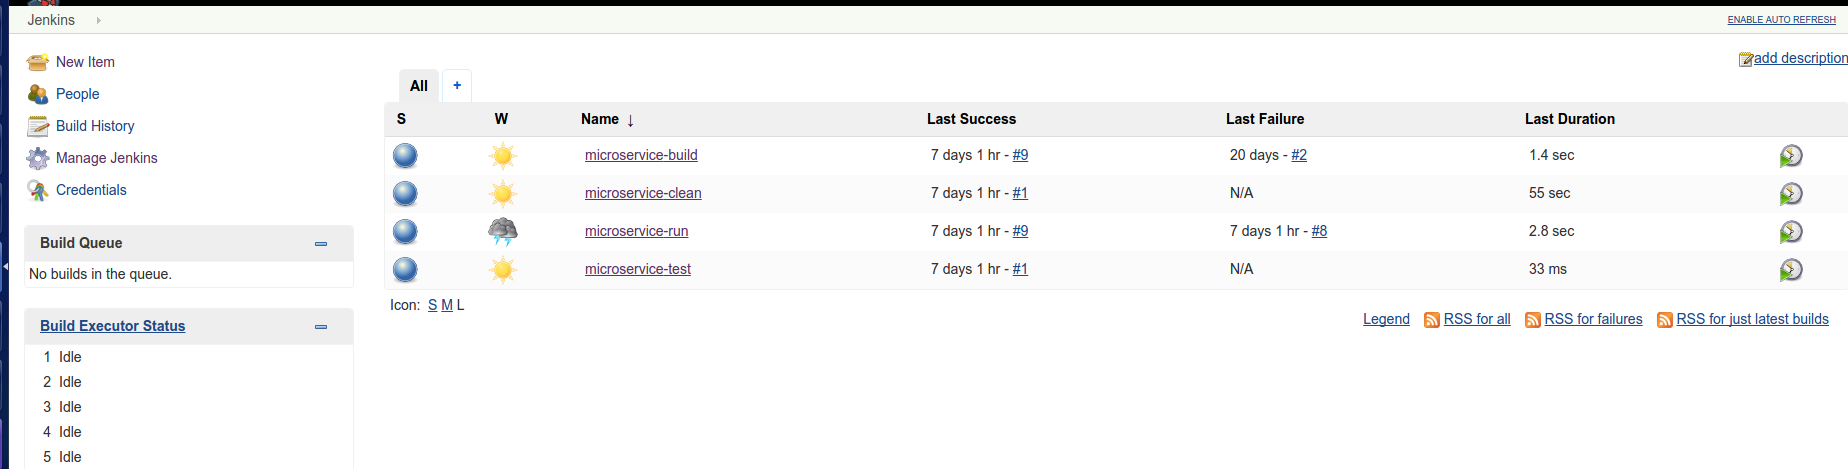
\includegraphics{img/jenkins-jobs.png}
\caption{Jenkins job-ok}
\end{figure}

\begin{itemize}
\tightlist
\item
  \textbf{bookstore-build}: Ennek a feladata a forrásfájlok és a Docker
  konténerek felkészítése. Miután a job végzett, a teljes infrastruktúra
  elkészíthető Docker konténerekből.
\end{itemize}

\begin{figure}[htbp]
\centering
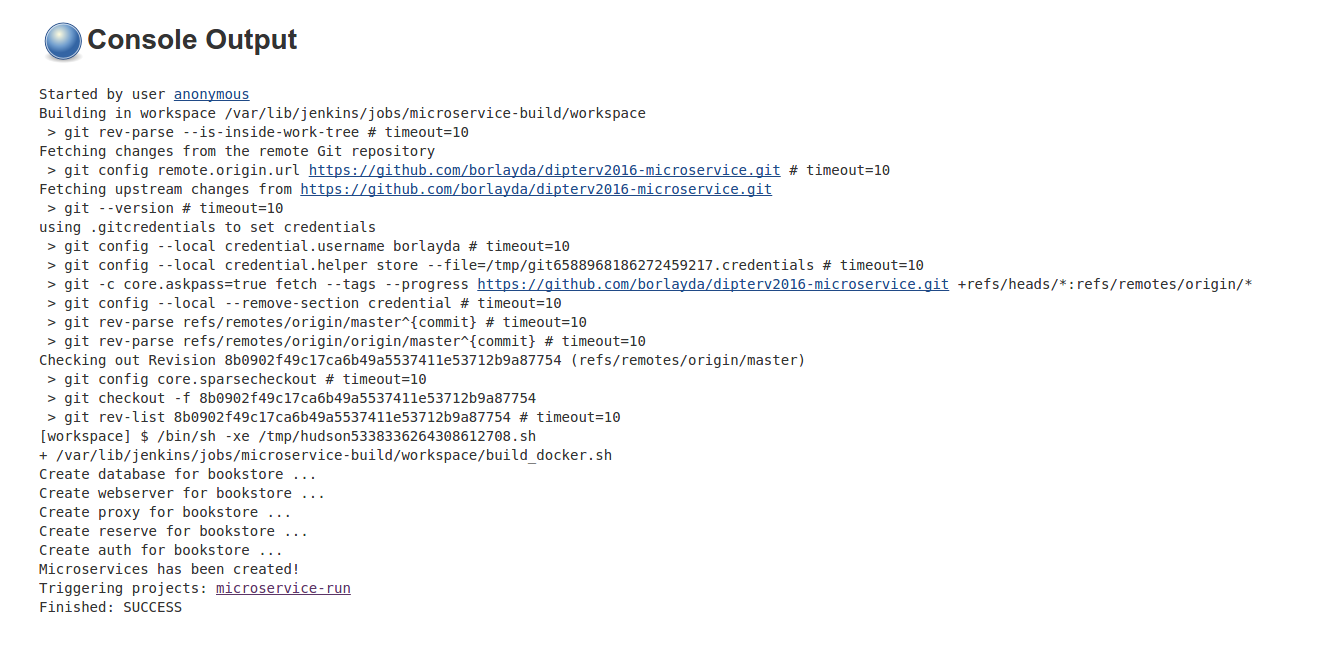
\includegraphics{img/jenkins-build.png}
\caption{Microservice build}
\end{figure}

\begin{itemize}
\tightlist
\item
  \textbf{bookstore-run}: Ennek a job-nak a feladata a Docker konténerek
  indítása, a szolgáltatások iniciaálizálása.
\end{itemize}

\begin{figure}[htbp]
\centering
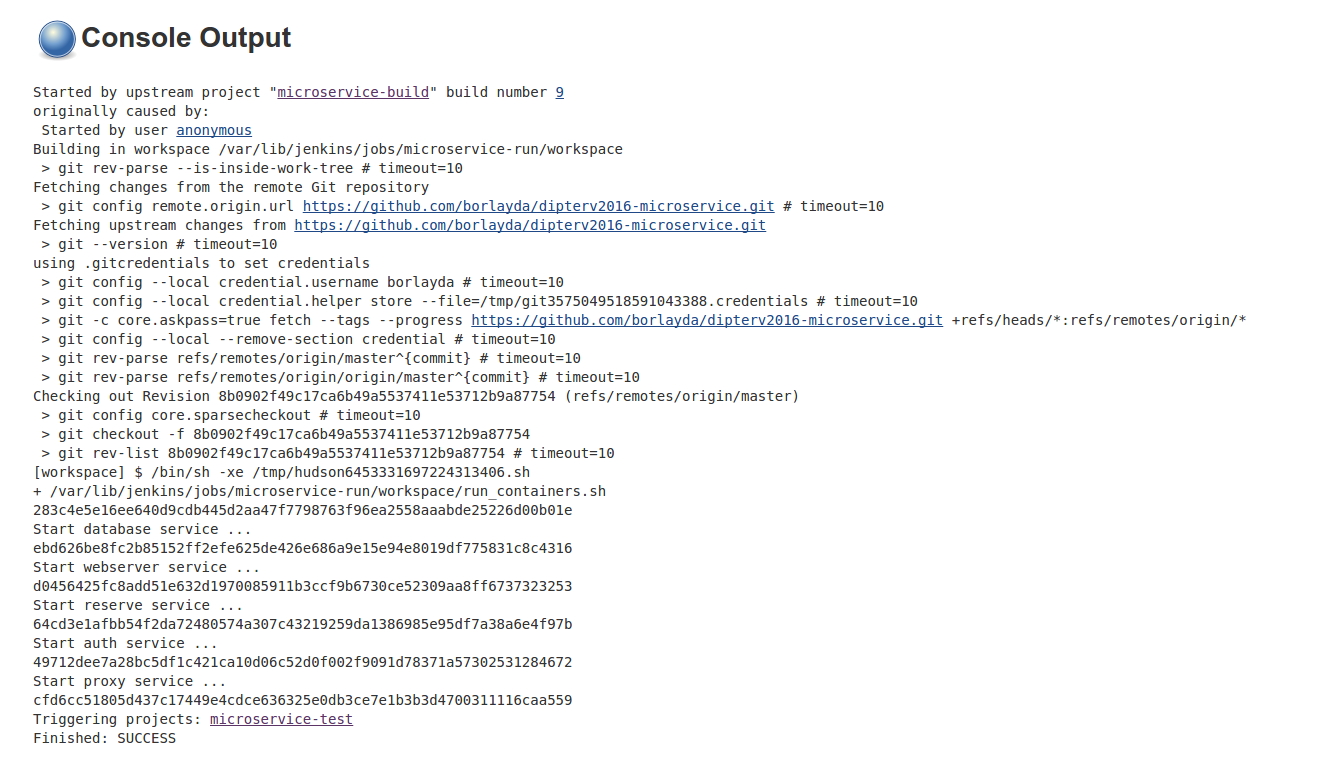
\includegraphics{img/jenkins-run.png}
\caption{Microservice run}
\end{figure}

\begin{itemize}
\tightlist
\item
  \textbf{bookstore-clean}: Ennek a job-nak a feladata, hogy a környezet
  ki legyen tisztítva, és ne maradjon a tesztek után semilyen Docker
  konténer, vagy fordított fájl a munkaterületen (workspace).
\end{itemize}

\begin{figure}[htbp]
\centering
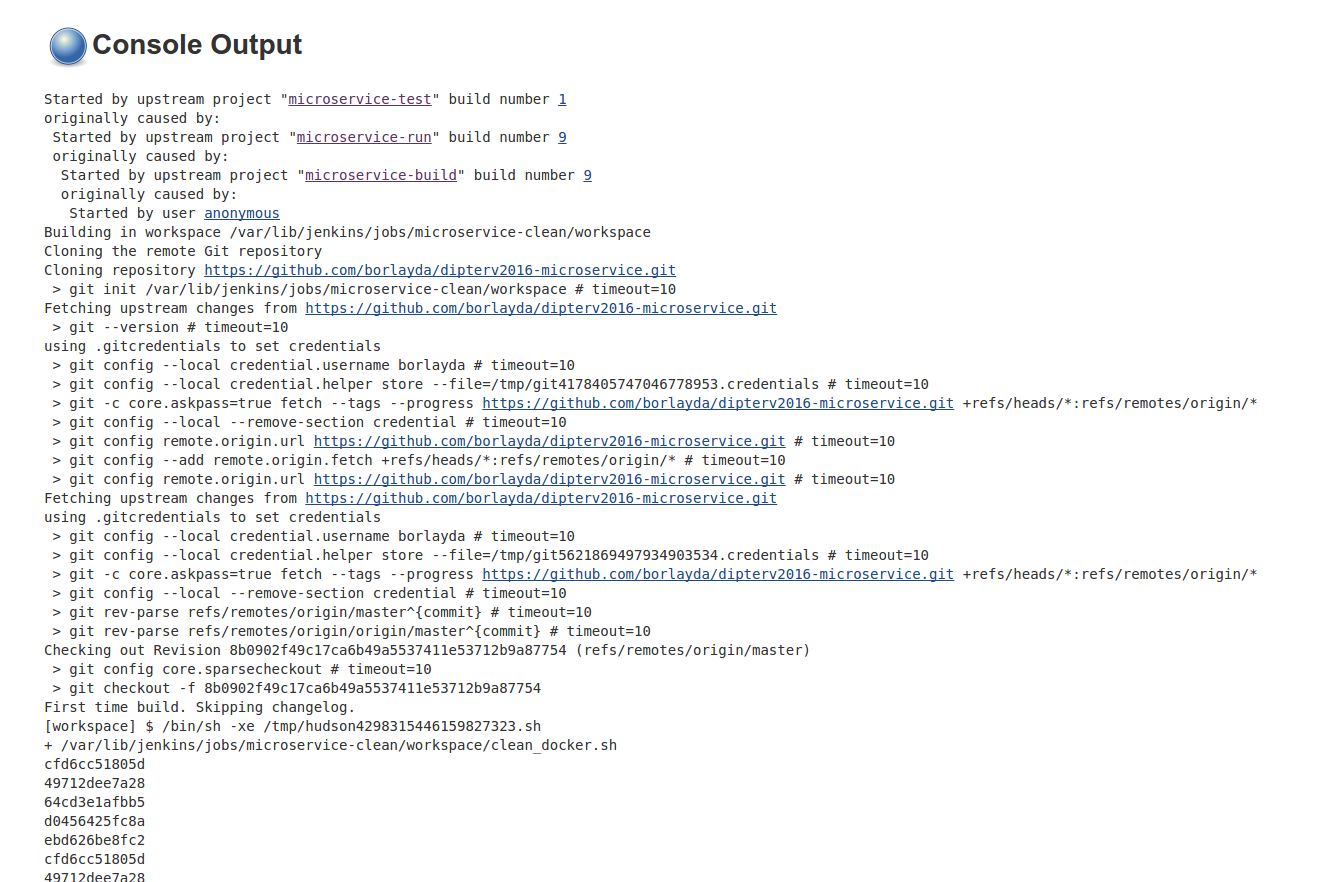
\includegraphics{img/jenkins-clean.png}
\caption{Microservice clean}
\end{figure}

\begin{itemize}
\tightlist
\item
  \textbf{bookstore-test}: Unit tesztek futtatása a feladata, de ide
  tartoznának a funkció és integrációs tesztek is, illetve a
  teljesítmény tesztek.
\end{itemize}

A Jenkins lehetővé teszi, hogy az egyes feladatok alfeladatokat
hívjanak, és egy komplex hierarchiát hozzanak létre. Ha bonyolultabb
vagy részletesebb felbontást szeretnék, csak fel kell vennem pár újabb
feladatot, és meg kell hívnom egy feladatból a többit.

\section{Egyéb minta
alkalmazások:}\label{egyuxe9b-minta-alkalmazuxe1sok}

KanBan board minta:

https://github.com/eventuate-examples/es-kanban-board

Archivematica minta:

https://www.archivematica.org/en/

\chapter{Összefoglaló}\label{uxf6sszefoglaluxf3}

A diplomaterv összefoglaló fejezete.

\listoftables
\listoffigures

\bibliography{bibliography}


\appendix

\chapter{Függelék}\label{fuxfcggeluxe9k}

\section{Dockerfile-ok}\label{dockerfile-ok}

\subsection{Authentikáció}\label{authentikuxe1ciuxf3}

Dockerfile.auth.service

\begin{verbatim}
FROM ubuntu
MAINTAINER Borlay Dániel <borlay.daniel@gmail.com>

COPY auth.sh /usr/sbin/auth.sh
COPY auth-service.py /usr/sbin/auth-service.py

RUN apt-get -y update
RUN apt-get -y install vim bash python-oauth python-mysqldb python \
    python-flask
RUN chmod +x /usr/sbin/auth.sh
RUN chmod +x /usr/sbin/auth-service.py

EXPOSE 8081
\end{verbatim}

\subsection{Proxy}\label{proxy}

Dockerfile.proxy.service

\begin{verbatim}
FROM haproxy
MAINTAINER Borlay Dániel <borlay.daniel@gmail.com>

COPY proxy.sh /usr/sbin/proxy.sh

RUN apt-get -y update
RUN apt-get -y install vim haproxy
RUN chmod +x /usr/sbin/proxy.sh
COPY haproxy.cfg /etc/haproxy/haproxy.cfg

ENTRYPOINT proxy.sh

EXPOSE 8080
\end{verbatim}

\subsection{Adatbázis}\label{adatbuxe1zis}

Dockerfile.database.service

\begin{verbatim}
FROM ubuntu
MAINTAINER Borlay Dániel <borlay.daniel@gmail.com>

COPY database.sh /usr/sbin/database.sh
COPY auth_init.sql /tmp/auth_init.sql
COPY bookstore_init.sql /tmp/bookstore_init.sql

RUN apt-get -y update
RUN apt-get -y install mysql-server mysql-client vim
RUN chmod +x /usr/sbin/database.sh
RUN sed -i 's/bind-address.*=.*/bind-address = 0.0.0.0/g' /etc/mysql/my.cnf

EXPOSE 3306
\end{verbatim}

\subsection{Vásárlás}\label{vuxe1suxe1rluxe1s}

Dockerfile.reserve.service

\begin{verbatim}
FROM centos
MAINTAINER Borlay Dániel <borlay.daniel@gmail.com>

COPY reserve.sh /usr/sbin/reserve.sh

RUN yum -y update
RUN yum -y install vim java-1.8.0-openjdk-devel tomcat7
RUN chmod +x /usr/sbin/reserve.sh

EXPOSE 8888
\end{verbatim}

\subsection{Webkiszolgáló
(böngészés)}\label{webkiszolguxe1luxf3-buxf6nguxe9szuxe9s}

Dockerfile.webserver.service

\begin{verbatim}
FROM httpd
MAINTAINER Borlay Dániel <borlay.daniel@gmail.com>

COPY webserver.sh /usr/sbin/webserver.sh
COPY index.html /var/www/html/index.html
COPY login.php /var/www/html/login.php
COPY store.php /var/www/html/store.php

RUN apt-get -y update
RUN apt-get -y install vim php5 php5-mysql curl php5-curl
RUN chmod +x /usr/sbin/webserver.sh

EXPOSE 80 443
\end{verbatim}

\section{Szkriptek}\label{szkriptek}

\subsection{Futtatáshoz}\label{futtatuxe1shoz}

\subsubsection{Build}\label{build}

build\_docker.sh

\begin{verbatim}
#!/bin/bash

services="database webserver proxy reserve auth"

for service in ${services}
do
    echo "Create ${service} for bookstore ..."
    mkdir -p services/${service}
    cp Dockerfiles/Dockerfile.${service}.service services/${service}/Dockerfile
    cp -R scripts/${service}/* services/${service}/
    docker build -t bookstore_${service} services/${service} \
      &> services/${service}/build.log
done

echo "Microservices has been created!"
\end{verbatim}

\subsubsection{Futtatás}\label{futtatuxe1s}

run\_containers.sh

\begin{verbatim}
#!/bin/bash

services="database webserver reserve auth proxy"

docker network create bookstore

for service in ${services}
do
    echo "Start ${service} service ..."
    docker run -d --name "${service}" -h "${service}" \
      --net=bookstore bookstore_${service} ${service}.sh "${DOCKER_IP_HAPROXY}"
done
\end{verbatim}

\subsubsection{Tisztogatás}\label{tisztogatuxe1s}

clean\_docker.sh

\begin{verbatim}
#!/bin/bash

services="database webserver proxy reserve auth"

docker stop $(docker ps -a | awk '/bookstore/ {print $1}')
docker rm $(docker ps -a | awk '/bookstore/ {print $1}')

for service in ${services}
do
    echo "Delete ${service} image"
    docker rmi bookstore_${service}
done

rm -rf services
docker network rm bookstore
\end{verbatim}

\subsection{Szolgáltatásokhoz}\label{szolguxe1ltatuxe1sokhoz}

\subsubsection{Adatbázis
inicializálás}\label{adatbuxe1zis-inicializuxe1luxe1s}

Authentikáció:

\begin{verbatim}
# Add permission to databases
GRANT ALL PRIVILEGES ON authenticate.* TO 'root'@'%';
GRANT ALL PRIVILEGES ON authenticate.* TO 'root'@'localhost';
# Create Tables
CREATE TABLE user_auth
(
    user_id int NOT NULL AUTO_INCREMENT,
    username varchar(255) NOT NULL,
    password varchar(255) NOT NULL,
    credential varchar(255),
    PRIMARY KEY (user_id)
);
# Fill Tables
INSERT INTO user_auth (username, password) VALUES ("test", "testpassword");
\end{verbatim}

Bookstore raktár:

\begin{verbatim}
# Add permission to databases
GRANT ALL PRIVILEGES ON bookstore.* TO 'root'@'%';
GRANT ALL PRIVILEGES ON bookstore.* TO 'root'@'localhost';
# Create Tables
CREATE TABLE store
(
    store_id int NOT NULL AUTO_INCREMENT,
    book_name varchar(255) NOT NULL,
    count int NOT NULL,
    PRIMARY KEY (store_id)
);
CREATE TABLE reservation
(
    reservation_id int NOT NULL AUTO_INCREMENT,
    username varchar(255) NOT NULL,
    book_name varchar(255) NOT NULL,
    count int NOT NULL,
    res_date varchar(255),
    PRIMARY KEY (reservation_id)
);
# Fill Tables
INSERT INTO store (book_name, count)
VALUES ("Harry Potter and the Goblet of fire", 10);
INSERT INTO store (book_name, count)
VALUES ("Harry Potter and the Philosopher's Stone", 10);
INSERT INTO store (book_name, count)
VALUES ("Harry Potter and the Chamber of Secret", 10);
INSERT INTO store (book_name, count)
VALUES ("Lord of the Rings: Fellowship of the ring", 3);
INSERT INTO store (book_name, count)
VALUES ("Lord of the Rings: The Two Towers", 3);
INSERT INTO store (book_name, count)
VALUES ("Lord of the Rings: The Return of the King", 0);
\end{verbatim}

\subsubsection{Bejelentkezéshez}\label{bejelentkezuxe9shez}

login.php:

\begin{verbatim}
<?php

if(!isset( $_POST['username'], $_POST['password']))
{
    echo 'Please enter a valid username and password';
}
else
{
    $username = filter_var($_POST['username'], FILTER_SANITIZE_STRING);
    $password = filter_var($_POST['password'], FILTER_SANITIZE_STRING);

    $ch = curl_init();
    curl_setopt($ch, CURLOPT_RETURNTRANSFER, true);
    curl_setopt($ch, CURLOPT_URL,
        "http://auth:8081/auth/{$username}/{$password}"
    );
    $content = curl_exec($ch);
    echo $content;
}
?>
\end{verbatim}

auth-service.py:

\begin{verbatim}
#!/usr/bin/env python
from flask import Flask, abort
import MySQLdb as mdb
app = Flask(__name__)

@app.route("/auth/<username>/<password>")
def hello(username, password):
    try:
        con = mdb.connect('database', 'root', '', 'authenticate');
        cur = con.cursor()
        cur.execute("SELECT user_id FROM user_auth \
                     WHERE username='%s' AND password='%s'" %
                     (username, password))
        user_id = cur.fetchone()
        print user_id
        if not user_id:
            abort(401)
    except mdb.Error, e:
        print "Error %d: %s" % (e.args[0],e.args[1])
        abort(401)
    finally:
        if con:
            con.close()
    return "Successfully authenticated!"

if __name__ == "__main__":
    app.run(host="0.0.0.0", port=8081)
\end{verbatim}

\subsubsection{Böngészés}\label{buxf6nguxe9szuxe9s}

index.html:

\begin{verbatim}
<html>
<head>
<title>Bookstore Microservice</title>
</head>
<body>

<h2>Login:</h2>
<form action="login.php" method="post">
  <fieldset>
    <p>
      <label for="username">Username</label>
      <input type="text" id="username" name="username" value=""/>
    </p>
    <p>
      <label for="password">Password</label>
      <input type="text" id="password" name="password" value=""/>
    </p>
    <p>
      <input type="submit" value="Login" />
    </p>
  </fieldset>
</form>

</body>
</html>
\end{verbatim}

store.php:

\begin{verbatim}
<html>
<head>
<title>Bookstore Microservice</title>
</head>
<body>

<h2>Books:</h2>

<table>
  <tbody>
    <tr><th>Name</th><th>Quantity</th></tr>

    <?php
      $servername = "database";
      $username = "root";
      $password = "";
      $dbname = "bookstore";

      // Create connection
      $conn = new mysqli($servername, $username, $password, $dbname);
      // Check connection
      if ($conn->connect_error) {
          die("Connection failed: " . $conn->connect_error);
      }

      $sql = "SELECT * FROM store";
      $result = $conn->query($sql);

      if ($result->num_rows > 0) {
          // output data of each row
          while($row = $result->fetch_assoc()) {
              echo "<tr><td>" . $row["book_name"]. \
              "</td><td> " . $row["count"]. "</td></tr>";
          }
      } else {
          echo "0 results";
      }
      $conn->close();
    ?>

  </tbody>
</table>

</body>
</html>
\end{verbatim}

Proxy config:

\begin{verbatim}
...
frontend web
    bind *:80
    mode http
    default_backend nodes

backend nodes
    mode http
    balance roundrobin
    server webserver webserver:80 cookie check
\end{verbatim}

\end{document}
